%!TEX root = /Users/markelikalderon/Documents/Git/formwithoutmatter/aristotle.tex
\chapter{The Eye} % (fold)
\label{cha:the_eye}

\section{The Soul of the Eye} % (fold)
\label{sec:the_soul_of_the_eye}

Sight, Aristotle tells us, is the soul of the eye,\index{sight!soul of the eye} or would be if it were an animal\index{animal}. This claim is made in the context of explaining what the soul of an animal is, and Aristotle proceeds by analogy with artifacts\index{artifact} and parts of animals:
\begin{quote}
	Suppose that a tool\index{tool}, e.g. an axe\index{axe}, were a natural body\index{body}, then being an axe would have been its essence\index{essence}, and so its soul\index{soul}; if this disappeared from it, it would have ceased to be an axe, except in name. As it is, it is an axe; for it is not of a body of that sort that what it is to be, i.e. its account, is a soul, but of a natural body of a particular kind, viz. one having in itself the power\index{power} of setting itself in movement and arresting itself. Next, apply this doctrine in the case of the parts of the living body. Suppose that the eye were an animal—sight would have been its soul, for sight\index{sight} is the substance\index{substance} of the eye\index{eye} which corresponds to the account, the eye being merely the matter\index{matter} of seeing\index{seeing}; when seeing is removed the eye is no longer an eye, except in name—no more than the eye of a statue\index{statue} or of a painted figure. (Aristotle, \emph{De Anima} \textsc{ii} 1 412\( ^{b} \)12--22; Smith in \citealt[22]{Barnes:1984uq})
\end{quote}

If an axe\index{axe} were a natural body, then what it is to be an axe would be both essential\index{essence} to the axe and its soul\index{soul}. If what it is to be an axe were somehow removed from a thing, then it would cease to be an axe. For a thing to have what it takes to be an axe is for that thing to possess a capacity for motion\index{motion} and rest characteristic of axes. Specifically, the thing must possess the capacity to cut in the manner of axes. If the thing had some other capacity, to join, for example, or if it cut in some other manner, then it would not be an axe, but a vice or a knife, say. Thus should a thing lose its capacity to cut, or to cut in that manner, it would cease to be an axe. It would be an axe in name only. The capacity to cut in the manner of axes is the essential form\index{form} and substance\index{substance} of an axe\index{axe}. If the capacity to cut in that manner is the form of an axe, then the material parts of the axe---the wooden shaft, the bronze head---constitute its matter\index{matter}. 

In the quoted passage, Aristotle notes an important limitation of the analogy. ``As it is, it is an axe.'' The essence\index{essence} of an axe\index{axe}, what it is to be an axe, is not in fact a soul. To conceive of an axe as a natural being is not yet to conceive of it as a living being. But living beings are the only natural beings with souls. An axe is merely conceived as a natural body\index{body} that contains within itself the power of motion and rest but not yet in the manner of a soul\index{soul}.

Aristotle's account of the soul of an axe conceived as a natural body is the model for his account of the soul of an eye conceived as an animal.\index{sight!soul of the eye} If an eye\index{eye} were an animal\index{animal}, then what it is to be an eye would be both essential to the eye and its soul. In supposing the eye to be an animal, a living being,\index{living being} the present analogy is not subject to the limitation of the previous analogy. If what it is to be an eye were somehow removed from a thing, then it would cease to be an eye. For a thing to have what it takes to be an eye is for that thing to possess the capacity for sight. Thus should a thing lose this capacity, it would cease to be an eye. It would be an eye in name only. A thing that lacks the capacity to see is like the eye of a statue, such as the drooping eye of King Seuthes \textsc{iii}\index{King Seuthes \textsc{iii}} in the 4th century \textsc{bc} Thracian bronze\index{bronze} portrait, the trace, perhaps of an old battle wound. The portrait is remarkably naturalistic, and the King's gaze is arresting. The artist used glass\index{glass} paste of different colors to distinguish the white of the eye\index{white of the eye}, the pupil\index{pupil}, and the iris\index{iris} and used thin copper\index{copper} wire for the eyelashes. Despite the striking naturalism and the intensity of the King's gaze, the drooping eye is, nonetheless, no real eye. Despite the naturalism and psychological expression achieved by the Thracian masterpiece, the colored glass paste, being opaque\index{opacity}, lacks the capacity to see\index{sight}. The capacity to see is the essential form\index{form} and substance\index{substance} of an eye. If the capacity to see is the form of the eye\index{eye}, then the material parts of the eye---the membrane, the interior water---constitute its matter\index{matter}.

% (see figure~\ref{fig:seuthesiii})
% \begin{figure}[htbp]
% 	\centering
% 		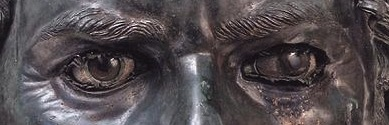
\includegraphics[scale=1]{graphics/seuthesiii.jpg}
% 	\caption{Detail of 4th century \textsc{bc} Thracian bronze portrait of King Seuthes \textsc{iii}}
% 	\label{fig:seuthesiii}
% \end{figure}

If we suppose the eye\index{eye} to be an animal\index{animal}, perhaps it makes sense to think of the hypothetical creature as possessing the capacity to see and so being the thing that sees, that exercises the capacity that it possesses. But if we relax that supposition, and consider an eye as it naturally occurs as part of an animal, then it would be wrong to think that an eye possesses the capacity to see. It is not the eye that sees but the animal that possesses that eye, or perhaps its soul. 

Plato\index{Plato} makes this point by means of an analogy: 
\begin{quote}
	\textsc{socrates}: Yes, my son. It would be a very strange thing, I must say, if there were a number of perceptions sitting inside us as if we were Wooden Horses, and there were not some single form, soul or whatever one ought to call it, to which all these converge---something \emph{with} which, \emph{through} those things, as if they were instruments, we perceive all that is perceptible. (Plato, \emph{Theaetetus} 184\( ^{d} \); Levett and Burnyeat in \citealt[204]{Cooper:1997fk})
\end{quote}
What is metaphorically described as the senses ``sitting inside us as if we were Wooden Horses'' is rejected as an unacceptable and is contrasted with an alternative where some one thing, the soul, perceives by means of the individual sense organs. Arethas of Caesarea\index{Arethas of Caesarea} suggested in the tenth century \textsc{ad} that the metaphorical description in the passage is an allusion to the Trojan horse\index{Trojan horse}. Recall, according to Homer\index{Homer}, the Achaeans\index{Achaeans} break the siege on Troy\index{Troy} by smuggling their warriors into the city within the trunk of a Wooden Horse\index{Wooden Horse} apparently left behind as a tribute. This plausible suggestion has been taken up by a number of subsequent commentators. If we accept that suggestion, then we can begin to elaborate the metaphorical description. The Achaean warriors hidden in the trunk of the Wooden Horse are capable of operating independently of one another and of the Wooden Horse in which they are contained. Similarly, the special senses\index{special senses} whose organs are parts of an animal's\index{animal} body would be understood to operate independently of one another and of the animal of whom they are a part. So conceived, the senses are what sense---the eye sees, and the tongue tastes. This, at any rate, is a consequence of the Heraclitean conception of perception\index{Heraclitus!perception}\index{Heraclitus!perception} involved in the Secret Doctrine\index{Secret Doctrine} (see \citealt[30--31]{Burnyeat:1976ab}). Moreover, while the Wooden Horse\index{Wooden Horse} may contain the Achaean warriors, it makes no use of them, and they do not operate as its instruments. Similarly the animal\index{animal} or its soul\index{soul} could make no use of the senses if they operated independently of one another and the animal of which they are a part. The Wooden Horse\index{Wooden Horse} would remain insensate despite being inhabited by warrior senses so conceived \citep[see][30]{Burnyeat:1976ab}. If the senses make us sensate, then they could not themselves possess the power to perceive, rather they must endow the perceiver with that capacity. The capacity to see may inhere in a spatial magnitude, the eye, the organ of sight, but it is the animal, or perhaps its soul, that exercises that capacity in seeing. It is not the eyes that see, but the animal whose eyes they are. Thus his eyes may have endowed King Seuthes \textsc{iii}\index{King Seuthes \textsc{iii}} with the capacity to see, at least when he was alive, but they did not themselves possess this capacity. Similarly amputated eyes\index{amputated eyes}, eyes separated from the animal in which they naturally occur as parts, neither possesses the capacity to see nor endow anything else with that capacity. 

There are thus grounds for criticizing a commitment of Empedocles\index{Empedocles} that arises in a passage that, as \citet[211]{Wright:1981zr}\index{Wright, M.R.} observes, Aristotle finds sufficiently interesting to cite three times (in \emph{De Anima} \textsc{iii}.6 430\( ^{a} \)27, \emph{De Caelo} \textsc{iii} 2 300\( ^{b} \)25, and \emph{De Generatione Animalium} \textsc{i} 18 722\( ^{b} \)17):
\begin{verse}
	as many heads without necks\index{heads without necks} sprouted up\\
	and arms wandered naked, bereft of shoulders\index{arms wandering naked, bereft of shoulders},\\
	and eyes roamed alone, impoverished of foreheads\index{eyes roaming alone, impoverished of foreheads}\\
	(Empedocles, \textsc{dk} 31\textsc{b}57; \citealt[64 245]{Inwood:2001ve})
\end{verse}
At a certain stage of the cosmic cycle, where Strife\index{Empedocles!Strife} still dominates but whose influence is on the wane as Love\index{Empedocles!Love} grows stronger, the parts of animals arise spontaneously and in a disordered state. These combine to give rise to fantastical animals, some with clear mythological precedent:
\begin{verse}
	Many with two faces and two chests grew,\\
	oxlike with men's faces,\index{oxlike with men's faces} and again their came up\\
	androids with ox-heads\index{androids with ox-heads}, mixed in one way from men\\
	and in another way in female form, outfitted with shadowy limbs.\index{hermaphrodite}\\
	(Empedocles, \textsc{dk} 31\textsc{b}61; \citealt[66 247]{Inwood:2001ve})
\end{verse}
These animals tended not to survive. It is only when animal parts are combined in harmony\index{harmony}, due to the increased influence of Aphrodite's\index{Aphrodite} Love\index{Empedocles!Love}, do the animals\index{animal} that we presently recognize emerge. Due to the harmony among their parts which fits them to a life in their natural environment, present animals not only survive but have the means of reproduction\index{reproduction}. Now consider the eyes roaming alone, impoverished of foreheads\index{eyes roaming alone, impoverished of foreheads}. Like amputated eyes\index{amputated eyes}, they are separated from animals in which they would harmoniously\index{harmony} occur as parts. And like amputated eyes, they neither possess the capacity to see nor endow anything else with that capacity. Though eye-like in structure and composition, these are eyes in name only, at least by Aristotle's lights:
\begin{quote}
	What a thing is is always determined by its function: a thing really is itself when it can perform its function; an eye, for instance, when it can see. When a thing cannot do so it is that thing only in name, like a dead eye or one made of stone, just as a wooden saw is no more a saw than one in a picture. (Aristotle, \emph{Meterologica} \textsc{iv} 12 390\( ^{a} \)10--14; Webster in \citealt[86]{Barnes:1984uq})\index{Meterologica@\emph{Meterologica}}
\end{quote}

The capacity to cut in the manner of axes is a power\index{power} and potentiality\index{potential}. A thing may possess this power, and so retain the potential to cut in that manner, even when at rest, when it is not actually cutting anything. Similarly, the capacity to see\index{sight} is a power and potentiality. A thing may possess or endow this power, and so retain the potential to see, even when at rest, when it is not actually seeing anything, because of darkness\index{dark} or sleep, say. Aristotle also claims that, in general, matter\index{matter!as potentiality} is potentiality and that form is actuality\index{form!as actuality}. There is no inconsistency here as the actual and the potential are said of in many ways. A thing is actually an axe\index{axe} if it possesses what it takes to be an axe, the capacity to cut in the manner of axes, the form and substance of an axe. Moreover the material parts of the thing, the matter\index{matter} of the axe---the wooden shaft, the bronze\index{bronze} head---are potentially an axe since they are capable of taking on the form of an axe. When the bronze is suitably fashioned, and honed, and securely fixed to the wooden shaft, the matter, in taking on the form that it does, in so acquiring the capacity to cut in the manner of axes, realizes this potentiality. But what it is to be an actual axe is itself a power\index{power} and potentiality\index{potential}, the capacity to cut in the manner of axes, a potentiality actualized in so cutting. Similarly, a thing is actually an eye if it possesses what it takes to be an eye, the capacity to see, the form and substance of an eye. Moreover the material parts of the thing, the matter\index{matter} of the eye\index{eye}---the membrane\index{membrane}, the internal water\index{internal water}---are potentially an eye since they are capable of taking on the form of an eye. When interior water is bound by the membrane and the other parts of the eye are suitably arranged, and the eye is harmoniously\index{harmony} related to the whole and healthy animal, the matter in taking on the form that it does, in so acquiring the capacity for sight, actualizes this potentiality. What it is to be an actual eye is itself to possess or endow a power and potentiality, the capacity to see, a potentiality actualized in seeing.

The actual and the potential are said of in many ways. In his discussion of these analogies, Aristotle distinguishes two senses of the actual/potential distinction. There is an initial potentiality had by some matter.\index{matter!as potentiality} This potentiality is realized by that matter taking on a form.\index{form!as actuality} The taking on of the relevant form is the first actuality\index{actual!first}. However, in the cases at hand, the relevant form is understood as the possession, or perhaps the endowment of, a capacity. So the first actuality is itself a potentiality. The realization of this potentiality, the exercise of the capacity which is the form of the matter, is the second actuality. These distinctions are schematically represented in table~\ref{tab:potential}

\begin{table}[htbp]
	\footnotesize
	\centering
		\begin{tabular}{cccc}
			& \emph{An Axe} & \emph{An Eye}\\
			\hline
			\emph{First Potenitality} & the matter of an axe & the matter of an eye\\
			\hline
			\emph{First Actuality/Second Potentiality} & the capacity to cut & the capacity to see\\
			\hline
			\emph{Second Actuality} & cutting & seeing\\
			\hline
		\end{tabular}
	\caption{Two senses of the actual/potential distinction}
	\label{tab:potential}
\end{table}

Eyes\index{eye} endow animals\index{animal} that possess them with the capacity to see.\index{sight} This is a capacity that animals enjoy even when asleep or inattentive. Endowing the perceiver with the capacity for sight is what the organ of sight is for. As \citet{Johansen:1997zr}\index{Johansen, T.K.} argues, this further teleological claim motivates a certain explanatory strategy with respect to the anatomical structure of the eye, what he describes as a ``top-down explanation''. Begin with what the organ of sight is for, to endow its possessor with the capacity to see. If the perceiver is endowed with this capacity, then the primary objects of sight, the colors of remote external particulars, potentially appear in the perceiver's experience of them. In order for the colors of remote external particulars to appear in the perceiver's experience of them, the organ of sight must be transparent. Sight is a reactive capacity, the organ of sight must be acted upon for sight to be exercised. And color only ever acts, even mediately, upon what is actually transparent. The eye has the structure and composition that it does to sustain the transparency\index{transparency} necessary to endow the perceiver with the capacity for sight. So our initial discussion of transparency (chapter~\ref{cha:transparency}) was necessary not only to understand Aristotle's definition of color\index{color!definition} (chapter~\ref{cha:color}) but also to understand Aristotle's explanatory strategy with respect to the anatomical structure of the eye. And understanding Aristotle's explanatory strategy, here, will yield insight into the significance of its limitations. Moreover, and importantly, understanding transparency is necessary to understand the way that the organ of sight must be acted upon if its possessor may see by means of it.

% section the_soul_of_the_eye (end)

\section{Transparency and the Anatomy of the Eye} % (fold)
\label{sec:transparency_and_the_anatomy_of_the_eye}

Why must the organ of sight be transparent?\index{eye!transparency}

Sight\index{sight} is a reactive capacity\index{capacity!reactive}. It is a mode of sensitivity\index{sensitivity} to the colors of remote external particulars\index{particular}. It only acts by reacting to the presence of a particular's color. Since sight is a reactive capacity, it must be acted upon in order for it to be exercised. That its exercise, an episode of seeing, just is being acted upon in this way is a further claim, that Aristotle denies, \emph{De Anima} \textsc{ii} 5. (For a contemporary defense of this denial see \citealt{Travis:2009fk} and \citealt{Kalderon:2012fk}.) Color could not immediately act upon the eye, since contact would blind the perceiver to the particular and its color. Contact precludes sensation, to be palpable is to be imperceptible.\index{to be palpable is to be imperceptible} Nevertheless, the color of a remote external particular can act upon the eye mediately, by acting upon the intervening medium. Thus was the moral of Aristotle's criticism of Democritus\index{Democritus} and Empedocles\index{Empedocles} (chapter~\ref{sec:against_the_empedoclean_principle}). The eye is itself affected by the color's effect on light\index{light}. Since color\index{color} is the power to alter what is actually transparent, the eye is affected by color's effect on transparent media by itself being transparent, at least in part. They eye is transparent, then, at least in part, so that the colors of remote external particulars may mediately act upon it. Which they must be capable of doing, since sight is a reactive capacity, a mode of sensitivity to the colors of remote external particulars arrayed in the natural environment.

Suppose that is right. Suppose that sight could only be the reactive capacity\index{capacity!reactive} that it is, a chromatic sensitivity\index{sensitivity}, if the organ of sight were transparent,\index{transparency} at least in part. This would constrain its elemental\index{elements} composition. Whereas some elements are receptive to the presence and activity of the fiery substance\index{fiery substance}, such as air\index{air} and water\index{water}, other elements, such as earth\index{earth}, exclude the fiery substance or at least retard its activity. Transparency\index{transparency} is present only in matter with a certain elemental composition, one that allows for the presence and activity of the fiery substance.

That sight\index{sight} is a reactive capacity\index{capacity!reactive}, a chromatic sensitivity\index{sensitivity}, not only constrains the elemental\index{elements} composition of the eye\index{eye}, but it also constrains its structure. Transparency is a nature\index{nature} or power\index{power} common to different substances such as water\index{water} and air\index{air}. So the requirement that the internal medium\index{medium!internal} of the eye\index{eye} be transparent\index{transparency} does not by itself determine whether an eye must have either elemental composition. Further material considerations determine that the internal medium be water:
\begin{quote}
	True, then, the visual organ proper is composed of water, yet vision appertains to it not because it is water, but because it is transparent---a property common alike to water and to air. But water is more easily confined and more easily condensed than air; it is that the pupil, i.e. the eye proper, consists of water. (Aristotle, \emph{De Sensu} \textsc{ii} 438\( ^{a} \)13--18; Beare in \citealt[5]{Barnes:1984uq})\index{De Sensu@\emph{De Sensu}}
\end{quote}
Air\index{air} and water\index{water} are liquids\index{liquid} and so lack fixed boundaries\index{unbounded}. If the organ of sight\index{eye} is thus composed, at least in part, of the transparent,\index{transparency} this liquid must somehow be confined to the organ of sight, by a fine membrane\index{membrane} (like the membrane\index{Empedocles!membrane} with which Aphrodite's\index{Aphrodite} Love\index{Empedocles!Love} enshrouds the primeval fire\index{fire} in the eye's\index{eye} interior, Empedocles\index{Empedocles} \textsc{dk} 31\textsc{b}84). That this is more easily done with water\index{water} than air\index{air} favors the conclusion that the eye\index{eye} is composed, at least in part, of water\index{water}. However, what is presently important is that reflection on the material constraints of sustaining an internal transparent medium\index{medium!internal} not only determines the elemental composition of the internal medium but also significant anatomical structure, the existence of a membrane that confines and condenses the internal water\index{internal water}.

That the eye\index{eye} is composed of water, at least in part, receives additional empirical support from gross anatomical observation\index{gross anatomical observation}. Water\index{water} flows from decomposing eyes\index{decomposing eyes} (\emph{De Sensu} \textsc{ii} 438\( ^{a} \)17)\index{De Sensu@\emph{De Sensu}}, and this water\index{water} is remarkably cold\index{cold} and glistening when it flows from the eyes of embryos\index{embryo} (\emph{De Sensu} \textsc{ii} 438\( ^{a} \)18). Whereas in sanguineous animals, the eye contains fat\index{fat} and oil\index{oil} to prevent the water\index{water} from freezing, the eyes of bloodless animals are covered for the the same reason (\emph{De Sensu} \textsc{ii} 438\( ^{a} \)20--3).


Aristotle's anatomy of the eye recapitulates important aspects of the ingestion model\index{ingestion model}, as presented in the answer in the style of Gorgias\index{Empedocles!answer in the style of Gorgias} (\emph{Meno} 76\( ^{a-d} \)):\index{Meno@\emph{Meno}}\index{Empedocles!lantern analogy}
\begin{quote}
	Now, as vision outwardly is impossible without light\index{light}, so also it is impossible inwardly. There must, therefore, be some transparent\index{transparency} medium\index{medium} within the eye\index{eye}, and, as this is not air\index{air}, it must be water\index{water}. The soul\index{soul} or its perceptive part\index{soul!perceptive part within} is not situated at the external surface\index{surface} of the eye\index{eye}, but obviously somewhere within: whence the necessity of the interior of the eye being transparent\index{transparency}, i.e. capable of admitting light. And that it is so is plain from actual occurrences. It is matter of experience that soldiers wounded in battle by a sword slash on the temple,\index{wounded soldier} so inflicted as to sever the passages of the eye\index{passages of the eye}, feel a sudden onset of darkness\index{dark}, as if a lamp\index{lantern} had gone out; because what is called the pupil, i.e. the transparent, which is a sort of lamp, is then cut off. (Aristotle, \emph{De Sensu} \textsc{ii} 438\( ^{b} \)7--15; Beare in \citealt[6]{Barnes:1984uq})
\end{quote}
This passage is the culmination of a dialectic\index{dialectical argument} that began at \emph{De Sensu} \textsc{ii} 437\( ^{b} \)11.\index{De Sensu@\emph{De Sensu}} An explanation of vision in terms of the eye's fiery emission, attributed to Empedocles\index{Empedocles} and Plato\index{Plato} in the \emph{Timaeus}\index{Timaeus@\emph{Timaeus}}, is contrasted with the competing explanation of Democritus\index{Democritus} in terms of the eye's\index{eye} reflection\index{reflection}. The passage presents a complex dialectical refinement of the \emph{endoxa}.\index{endoxa@\emph{endoxa}} The explanations of Empedocles and Democritus are, of course, rejected. Importantly, however, Aristotle retains elements of each of their explanations, even if these elements are fundamentally reconceived.

According to Aristotle, Democritus\index{Democritus} maintains that the eye\index{eye} sees because of its reflective\index{reflection} surface\index{surface}, itself due to the smoothness\index{smooth} of the eye and the presence of lachrymal fluid\index{lachrymal fluid} (\emph{De Sensu} \textsc{ii} 438\( ^{a} \)5--12).\index{De Sensu@\emph{De Sensu}} Democritus is wrong in thinking that this was due to water's\index{water} capacity for reflection\index{reflection}, and consequently wrong in taking the locus of sight to be on the surface\index{surface} of the eye. Specifically, Democritus'\index{Democritus} account overgeneralizes---there are reflective\index{reflection} things that lack the capacity for sight\index{sight}. Nevertheless, Democritus was right to link the eye's capacity to see with the presence of water. However, it is not the reflectivity\index{reflection} but the transparency\index{transparency} of the eye's water\index{water} that is required to endow its possessor with the capacity to see. 

This parallels the way that Empedocles\index{Empedocles} accommodates the dominant medical opinion of his time (discussed in chapter~\ref{sec:empedocles_theory_of_vision}). The presence of lachrymal fluid\index{lachrymal fluid} is both necessary for sight\index{sight} and necessary for the reflective\index{reflection} appearance of the eye\index{eye}. This encouraged the opinion that the reflective appearance of the eye explained the eye's receptivity to sight, and hence that the surface of the eye is the locus of sight. However, on the ingestion model\index{ingestion model}, the assimilation\index{assimilation!material} of chromatic effluences\index{Empedocles!effluence!chromatic} is a material precondition for their presentation to the organ of sight. On the ingestion model, sight is located within. By conceiving of the receptors on the surface of the eye as water-bound passages to its interior, Empedocles reconciles the ingestion model\index{ingestion model} with the dominant medical opinion of his time. Similarly, Aristotle asserts that ``the soul or its perceptive part is \ldots\ obviously within'' (\emph{De Sensu} \textsc{ii} 438\( ^{b} \)9--10; Beare in \citealt[6]{Barnes:1984uq}).\index{soul!perceptive part within} And like Empedocles, Aristotle retains something of Democritus' opinion. But not by finding a role for the surface of the eye in seeing, but by claiming that the eye is partly composed of water. Moreover, as we shall see, the transparent plays a role similar to the role played by ocular passages in Empedocles's theory of vision.

Aristotle rejects the explanation of vision in terms of the eye's fiery emission\index{Empedocles!perception!fiery emission}. While Aristotle attributes this view to Empedocles on the basis of the lantern analogy\index{Empedocles!lantern analogy}\index{lantern} (\textsc{dk} 31\textsc{b}84; quoted in full at \emph{De Sensu} \textsc{ii} 437\( ^{b} \)27--438\( ^{a} \)3), he also writes:
\begin{quote}
	Sometimes he accounts for vision thus, but at other times he explains it by emanations from the visible objects. (Aristotle, \emph{De Sensu} \textsc{ii} 438\( ^{a} \)3--4; Beare in \citealt[5]{Barnes:1984uq})\index{De Sensu@\emph{De Sensu}}
\end{quote}
As discussed in chapter~\ref{sec:empedocles_theory_of_vision}, Aristotle thinks that Empedocles is potentially offering distinct explanations of color vision---one in terms of the eye's emission of fiery effluence\index{Empedocles!perception!fiery emission} and the other in terms of the eye's assimilation of chromatic effluences\index{Empedocles!effluence!chromatic}. While Aristotle rejects the explanation of color vision in terms of the eye's fiery emission, he reinterprets Empedocles' lantern analogy on the model of the answer in the style of Gorgias,\index{Empedocles!answer in the style of Gorgias} though with crucial refinements.

While rejecting the explanation of vision in terms of the eye's fiery emission, nowhere does Aristotle directly deny the fundamental claim of Empedoclean a\-nat\-o\-my that the eye is composed of ``fire and its opposite'' (Theophrastus\index{Theophrastus}, \emph{De Sensibus}, \textsc{xv}).\index{De Sensibus@\emph{De Sensibus}} Perhaps, this is not an omission on Aristotle's part but intentional, for there is another way to understand Empedocles talk of interior fire\index{internal fire}. If the eye's interior is composed of confined and condensed water\index{internal water} in order to sustain its transparency\index{transparency}, then the interior water, being transparent, is receptive to the presence and activity of the fiery substance\index{fiery substance}. The external medium\index{medium!external} must be illuminated if the color\index{color} of a remote external particular\index{particular} is to be visible in it. Similarly, for that color to be visible, the external light must be extended within. The transparent water of the eye's interior must itself be illuminated. And the internal medium\index{medium!internal} is only illuminated by the presence and activity of the fiery substance\index{fiery substance}. While seeing the white\index{white} of the sun\index{sun} may not involve the assimilation\index{assimilation!material} of fiery effluences as Empedocles\index{Empedocles} maintained, nevertheless, if the white of the sun is visible to the perceiver, this is due, in part, to the presence and activity of the fiery substance\index{fiery substance} in the eye's interior. This is why Aristotle makes the deliberate allusion to Empedocles' lantern analogy\index{Empedocles!lantern analogy} (\textsc{dk} 31\textsc{b}84). Like Empedocles, Aristotle compares the eye to a lantern\index{lantern}. But not because the eye\index{eye} emits fire\index{fire} the way a lantern does. But because the interior of the eye must be illuminated, the way the interior of a lamp is illuminated, if the external scene is to be visible. So not only does Aristotle retain the phenomenological insight of Empedocles, that seeing is a mode of assimilation, ``the soul or its perceptive part'' within.\index{soul!perceptive part within} But Aristotle also retains the Empedoclean doctrine that the exercise of the capacity for sight\index{sight} involves fire\index{fire} in the eye's interior, understood as the fiery substance\index{fiery substance} illuminating the internal medium\index{medium!internal}. 

Though Aristotle reinterprets Empedocles' lantern analogy\index{Empedocles!lantern analogy} on the model of the answer in the style of Gorgias,\index{Empedocles!answer in the style of Gorgias} there are crucial refinements, as he rejects the theory of effluences.\index{Empedocles!effluence} 

According to Empedocles\index{Empedocles}, what is assimilated is a material\index{assimilation!material} particular\index{particular}, a chromatic effluence,\index{Empedocles!effluence!chromatic} conceived as a fine body\index{body}, composed of fire\index{fire} or water\index{water}, with a distinctive magnitude\index{magnitude}. On Aristotle's reinterpretation of the lantern analogy\index{Empedocles!lantern analogy}, what is assimilated is not a material\index{assimilation!material} particular\index{particular}, but the state of the external medium\index{medium!external}, a state\index{state} sustained by the illuminating presence and activity of the fiery substance\index{fiery substance}. The state of the internal medium\index{medium!internal} need not be the same as the state of the external medium. Internal and external media may differ in their degree of transparency\index{transparency!degrees of}, and so dark eyes may be illuminated to a lesser degree than the surrounding air. Nevertheless, the state of illumination of the interior water\index{internal water} is determined by the amount of fiery substance\index{fiery substance} encountered in the external medium\index{medium!external} and the degree of transparency of the internal medium, the degree to which it is susceptible to the illuminating presence and activity of the fiery substance. 

Despite rejecting the theory of effluences\index{Empedocles!effluence}, the transparency\index{transparency} of interior water\index{internal water} plays, for Aristotle, a function that ocular passages play in Empedocles' theory of vision.\index{Empedocles!perception} Chromatic effluences,\index{Empedocles!effluence!chromatic} because of their distinctive magnitudes,\index{magnitude} are commensurate\index{Empedocles!perception!commensurate} with ocular passages\index{Empedocles!passage}. As such, they can travel through such passages and so be palpable to the organ of sight. While a state lacks location, and so cannot travel, the external light\index{light} is extended within, in the sense in which it can, so that the color of remote external particulars may be present in visual consciousness. It is thanks to the illuminated state of the eye's interior that the perceiver is able to assimilate the chromatic form of distal particulars in the natural environment. As I argued in chapter~\ref{sec:the_answer_in_the_style_of_gorgias}, the assimilation\index{assimilation!material} of chromatic effluences by the organ of sight is not, by itself, the sensing of colors. The assimilation of chromatic effluences is at best a material precondition for their sensing. Similarly, admitting light into the interior of the organ of sight is not, by itself, the sensing of colors. Interior illumination is at best a material precondition for their sensing. Sensing is the presentation of the color to the perceptive part of the soul, not by being palpable, but by the assimilation of chromatic form, by the color of remote external particulars shaping visual consciousness. However the doctrine of the assimilation of sensible form is to be understood, interior illumination is a material precondition for sensing, so understood. That the interior illumination takes on a character that depends upon and derives from the character of the exterior illumination may make the colors of remote external particulars perceptually available, but the perceptually availability of the colors only involves the colors being potentially perceived, not their actual perception.  

% This is another aspect of the ingestion model that is preserved in Aristotle's dialectical refinement of Empedocles' theory.

The present understanding of Aristotle's deployment of the lantern analogy\index{Empedocles!lantern analogy} is further confirmed by the empirical evidence that Aristotle marshals at the end of this passage (\emph{De Sensu} 438\( ^{b} \)12--15).\index{De Sensu@\emph{De Sensu}} That the eye\index{eye} must be ``capable of admitting light \ldots\ is plain from actual occurrences'', such as the blindness resulting from a wound sustained by a slash on the temple.\index{wounded soldier} Such a wound severs passages leading away from the eye\index{passages of the eye} and so impairs the eye's capacity to endow its possessor with sight. Though the wounded soldier's eyes are filled with light\index{light}, since the passages leading within are severed, presumably, to a position at or near the heart\index{heart}, the colors\index{color} of remote external particulars\index{particular} are no longer present in his visual consciousness. While they appear through the internal medium, being actually transparent, the colors of distal particulars are cut off from the perceptive part of the soul.\index{soul!perceptive part within} The wounded soldier\index{wounded soldier} can no longer assimilate the chromatic form of remote material particulars.

We have here another significant part of the eye's anatomy, the passages from the eye leading within.\index{passages of the eye} One should not anachronistically assume that Aristotle has in mind the optic nerve.\index{optic nerve} Given that the seat of sensation is at or near the heart\index{heart}, a better hypothesis would be that they are vessels\index{blood vessels} leading to the heart. However, Aristotle's description of these passages\index{passages of the eye} underdetermines any such identification \citep[see][]{Lloyd:1978fk}. In fact, Aristotle seems only interested in this anatomical detail insofar as these passages extends the transparent\index{transparency} within. In extending the transparent within, the perceptive part of the soul\index{soul!perceptive part within} becomes receptive to the direction of influence of the fiery substance\index{fiery substance!direction of influence}. It is the presence and activity of the fiery substance\index{fiery substance} that determines the sensible character of internal and external media\index{medium!external}\index{medium!internal}. Moreover, the sensible character of transparent media is itself determined by the colors\index{color} of the particulars\index{particular} that appear through that media. The precise content of the Aristotelian doctrine of the assimilation of sensible form\index{assimilation!of sensible form} remains, at this point, unclear. What is clear is that, first, it does not involve chromatic forms traveling in the manner of effluences, as \citet[\textsc{i} 1]{Hobbes:1651fk} imagined, and that second, the passages extending the eye's transparency within are necessary for the assimilation of chromatic form. 

Not only does Aristotle's empirical example provide us with another significant part of the eye's anatomy, but it also further illustrates what \citet{Johansen:1997zr}\index{Johansen, T.K.} describes as Aristotle's ``top-down explanation''. Sight\index{sight!soul of the eye} is the soul of the eye, or it would be if it were an animal\index{animal}. Endowing its possessor with the capacity for sight is what the organ of sight is for.\index{sight!for the sake of seeing} Consequently the organ of sight is understood to have the structure and composition required to endow this capacity. Evidently, passages extending the transparent within are necessary for the capacity for sight, since when they are severed, the victims of such wounds are blinded.\index{wounded soldier} We have an explanation from what the organ of sight is for---to endow the perceiver with the capacity for sight---to anatomically significant structure---passages leading away from the eye.

So far we have distinguished the condensed and confined water in the eye's interior,\index{internal water} the membrane\index{membrane} that confines it, the pupil\index{pupil}, and passages leading away from the eye\index{passages of the eye} to some point in the interior, perhaps, at or near the heart\index{heart}. In addition, Aristotle distinguishes the dark of the eye\index{dark of the eye|see{iris}} from the light\index{white of the eye} (\emph{De Sensu} \textsc{ii} 437\( ^{b} \)1),\index{De Sensu@\emph{De Sensu}} understood as the iris\index{iris} and the white of the eye\index{white of the eye} that surrounds the iris\index{iris} (\citealt[see][218, 231 n13]{Lloyd:1978fk}). In sanguineous animals, the white\index{white of the eye} is fat\index{fat} and oily\index{oil} to prevent the transparent\index{transparency} water\index{internal water} of the eye\index{eye} from freezing (\emph{De Sensu} \textsc{ii} 438\( ^{a} \)20--3). The contrast must be with the dark\index{dark} of the eye, as opposed to the black\index{black}, since Aristotle recognizes different colored irises\index{iris}: ``In some it is black\index{black}, in some distinctly blue\index{blue}, in some greyish-blue\index{grayish-blue}, in some greenish\index{greenish}'' (Aristotle, \emph{Historia Animalium} \textsc{i} 10 492\( ^{a} \)2--3\index{Historia Animalium@\emph{Historia Animalium}}; Thompson in \citealt[13]{Barnes:1984uq}). Blue\index{blue}, grayish-blue\index{grayish-blue}, and greenish\index{greenish} may be dark\index{dark}, at least when compared with the white of the eye\index{white of the eye}, but they are not black\index{black}. Further evidence, if any were needed, that \emph{melaton}\index{melaton@\emph{melaton}} and its cognates should be understood as dark\index{dark} as opposed to black\index{black} in the Aristotelian color scheme.

% \begin{figure}[htbp]
% 	\centering
% 		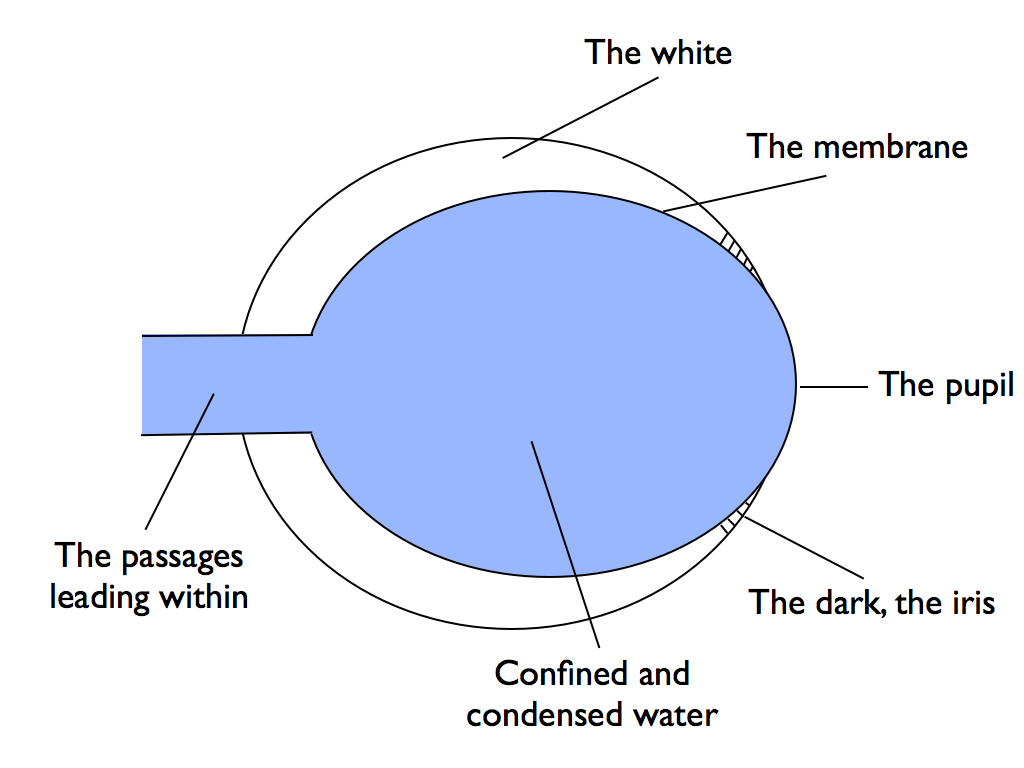
\includegraphics[scale=0.3]{graphics/eye.jpg}
% 	\caption{Aristotelian anatomy of the eye}
% 	\label{fig:eye}
% \end{figure}

The Aristotelian anatomy of the eye is crude, even by ancient standards. Lloyd summarizes its limitations:
\begin{quote}
	Yet no attempt is made to describe the structure of the eye as a whole, although this is, of course, complex. The three main parts Aristotle identifies quite incidentally in the course of this chapter, pupil, iris, white, relate primarily to the superficial appearance of the eye. Apart from the one reference to the membrane of the eye and the one reference to certain \emph{poroi}, already mentioned, his remarks on the internal structure of the eye are confined to the point that the pupil, \emph{kore}, consists of water. We may take it that this refers to the vitreous humour that occupies most of the bulb of the eye and which, in certain lesions, might produce a watery discharge. But there is no mention of the membrane enveloping the vitreous humour (retina, choroid, sclera), nor of the lens, nor of the anterior chamber between the cornea and the lens. There is, in fact, no mention of most of the parts that seem difficult to identify straightforwardly as water, and no systematic description of the internal structure of the eye as such at all. \citep[220--221]{Lloyd:1978fk}\index{Lloyd, G.E.R.}
\end{quote}
While the Aristotelian anatomy of the eye can be further refined and extended (and was by the commentators---Philoponus\index{Philoponus, John} recognized the anterior chamber\index{eye!anterior chamber} between the cor\-nea\index{cornea} and the lens\index{lens}), important limitations will inevitably remain. The significance of these limitations should be judged in relation to the specific explanatory concerns Aristotle and the Peripatetic tradition were addressing in articulating the eye's\index{eye} anatomy. \citet{Lloyd:1978fk}\index{Lloyd, G.E.R.} takes Aristotle to be primarily addressing the problem of how to assign the four elements\index{elements} to the five senses\index{special senses}. This is indeed a task of \emph{De Sensu}\index{De Sensu@\emph{De Sensu}}. But, as I have argued, Aristotle has more specific explanatory concerns. The eye must have such a nature so as it may be mediately acted upon by color in order to endow its possessor with the reactive capacity\index{capacity!reactive} for sight\index{sight}. Taken by itself, this claim is the expression of a reasonable explanatory strategy. If Aristotle's anatomy of the eye\index{eye} strikes us as superficial or schematic, this is not due to this explanatory strategy alone, nor is it due to an abstract taxonomic concern with assigning elements to senses. Rather, two further claims are responsible for the limitations of Aristotelian anatomy: (1) that the eye\index{eye} can only be mediately acted upon if it is actually transparent\index{transparency}, and (2) that the eye is only acted upon by altering the character of its interior illumination\index{light}. Whereas (1) specifies a condition on the patient of change, (2) specifies the nature of the change. It is these further commitments that lead him to discern only those parts of the eye that might plausibly be said to play a role in sustaining the transparency of the internal medium\index{medium!internal}.


% section transparency_and_the_anatomy_of_the_eye (end)

\section{Interior Illumination} % (fold)
\label{sec:interior_illumination}

The eye\index{eye} in seeing is like a lantern\index{lantern}\index{Empedocles!lantern analogy}, not because it emits fire\index{Empedocles!perception!fiery emission} from its interior, but because in seeing the interior of the eye is illuminated. The confined and condensed water\index{internal water} in the interior of the eye is transparent\index{transparency} for the sake of receiving such illumination. It is only be being transparent that colors can mediately act upon the eye by acting upon the intervening medium. And since sight is a reactive capacity\index{capacity!reactive}, a mode of chromatic sensitivity\index{sensitivity}, the organ of sight must be acted upon if the capacity for sight is to be exercised in seeing the presented color.

What is the effect that the color produces in mediately acting upon the eye?

Since color acts upon the eye by acting upon the external me\-di\-um, the effect on the internal medium\index{medium!internal} should be of the same kind as the effect that color has on the external medium\index{medium!external}. Aristotle explicitly speaks of admitting light\index{light}. Colors affect the character of the illuminated medium, so in admitting light, the transparent\index{transparency} medium within the eye\index{eye} not only must be actually transparent, due to the illuminating presence and activity of the fiery substance, but it must also come to have a character that at least corresponds to the character of the external illuminated medium. The correspondence need not be identity. As we observed, internal\index{medium!internal} and external media\index{medium!external} may differ in their degree of transparency\index{transparency}, and so dark\index{dark} eyes may be illuminated to a lesser degree than the surrounding air. The light\index{light} admitted by dark eyes, their interior illumination, will not be as bright as the exterior illumination. Nevertheless, the existence and character of the interior illumination depends upon and derives from the existence and character of the external illumination that immediately acts upon it.

This places an important metaphysical constraint on the character of the interior illumination. Whatever effect color\index{color} has on the external medium\index{medium!external}, such as the surrounding air\index{air}, the external medium has a corresponding effect on the internal medium\index{medium!internal}. In chapter~\ref{sec:the_definition_of_color}, we reviewed some candidate effects. Given the metaphysical constraint, the candidate effects on the internal medium, the illuminated water in the eye's\index{eye} interior,\index{internal water} correspond to these.

In chapter~\ref{sec:the_definition_of_color}, I argued that color\index{color} could not color external media\index{medium!external} since doing so would be inconsistent with the way that colors are perceptually available within them---either by being inconsistent with the medium being actually transparent or by being inconsistent with the directionality of the visible\index{the visible!directionality of}. The agent of a change must actually be the way that the patient potentially is. Insofar as the external medium\index{medium!external} acts upon the internal medium\index{medium!internal}---light\index{light} is admitted---the external medium is an agent of change, the internal medium the patient. Since the external medium could not be colored, in admitting light, the internal medium, the transparent\index{transparency} water within\index{internal water} the eye's interior, could not in turn be colored. This result is one of the advantages of the present mode of exposition, focused fundamentally on the nature of the transparent, that begins with color's effect on external transparent media before considering color's mediate effect on internal transparent media.

In chapter~\ref{sec:the_definition_of_color}, I also rejected Burnyeat's\index{Burnyeat, M.F.} suggestion that the illuminated medium is not genuinely altered but merely undergoes a quasi-alteration\index{quasi-alteration} when acted upon by color\index{color}. I argued that quasi-alteration was perhaps too Protagorean\index{Protagoras} to be genuinely of Aristotelian provenance. It was, in any case, undermotivated. Burnyeat's\index{Burnyeat, M.F.} case for quasi-alteration\index{quasi-alteration} depended upon the thought that the medium\index{medium} could not be materially altered by the colors arrayed in it consistent with the perspective relativity\index{perspective} of the perceptual availability of the colors\index{color}. However, I argued that if color acts upon the illuminated medium\index{medium} by promoting or retarding the activity of the fiery substance\index{fiery substance} illuminating it, then that medium undergoes a material change that is not only consistent with the directionality of the visible\index{the visible!directionality of}, but provides an explanation for it. The being of fire\index{fire} consists in its burning. Burning is an activity. And, as such, it has a direction of influence. That the perceptual availability of a color depends upon the perceiver’s point of view is due,\index{perspective} in part, to the direction of influence that results from that particular’s color altering the activity of the fiery substance.\index{fiery substance!direction of influence}

As before, three candidate effects remain:
\begin{enumerate}[(1)]
	\item the rendering visible of the transparent---making the transparent internal me\-di\-um perceptually available;
	\item the rendering visible of colored particulars arrayed in the transparent external me\-di\-um\----making the colored particulars perceptually available; and
	\item affecting the fiery substance by affecting the amount of it in the internal me\-di\-um, the water within the eye, or, if this does not come to the same thing, promoting or retarding its activity to some degree, or otherwise affecting its direction of influence
\end{enumerate}

(1) follows from the \emph{De Anima} (\textsc{ii} 7 418\( ^{b} \)4--6)\index{De Anima@\emph{De Anima}} definition of the transparent\index{transparency!definition}. It might seem odd to claim that the transparent water\index{internal water} in the eye's\index{eye} interior is perceptually available to us, even when illuminated. However, recall, by Aristotle's definition of transparency\index{transparency!definition}, the transparent appears to us by the colors\index{color} of remote external particulars\index{particular} appearing through it\index{perception!at a distance}. Since when we see the colors of remote external particulars, we see them through the transparent medium\index{medium!internal} in the eye's\index{eye} illuminated interior, we see that medium as well. Of course, ordinarily we do not attend to the transparency of the eye's interior water until it is disrupted, when we see floaters, say. But, in seeing the colors, the internal medium must itself be perceptually available, at least in the manner of transparent things enshrined in the \emph{De Anima}\index{De Anima@\emph{De Anima}} definition of transparency\index{transparency!definition}. 

(2) is not only a consequence of the \emph{De Anima}\index{De Anima@\emph{De Anima}} definition\index{transparency!definition}, but is a commitment of Aristotle's description of the wounded soldier\index{wounded soldier}. That the colored\index{color} particulars\index{particular} arrayed within the transparent\index{transparency} external medium\index{medium!external} are perceptually available within the water in the eye's interior is demonstrated by severing the illuminated interior from the perceptive part of the soul, located at or near the heart. When the transparency in the eye's interior is no longer extended within, the passages leading from the eye having been severed by a sword's blow, the colors of remote external particulars are no longer perceptually available. The soldier has been blinded by his wound. 

(3) not only draws upon materials available in both \emph{De Anima}\index{De Anima@\emph{De Anima}} and \emph{De Sensu}\index{De Sensu@\emph{De Sensu}}, but coheres well with the \emph{De Sensu} project of explaining what each of the sense object must be to produce the sensation in full actuality. Moreover, (3) is directly involved in Aristotle's reinterpretation of Empedocles' lanterns analogy\index{Empedocles!lantern analogy}. The eye\index{eye} is like a lantern\index{lantern}, not because it emits fire, but because its interior is illuminated. Not only does the potentially transparent water in the eye's interior become actually transparent\index{transparency}, but it comes to have a character that at least corresponds to the character of the external illumination. The existence and character of interior illumination depends upon and derives from the existence and character of the external illumination that immediately acts upon it. Specifically, the existence and character of the interior illumination will depend upon the amount, degree of activity, and direction of influence of the fiery substance\index{fiery substance!direction of influence} encountered in the external medium\index{medium!external} and the internal medium's\index{medium!internal} degree of transparency\index{transparency!degrees of}, the degree to which it is receptive to the illuminating presence and activity of the fiery substance\index{fiery substance}. So understood, (3) is not only consistent with, but explanatory of, (1) and (2). In becoming actually transparent, objects can be seen through that medium. Interior illumination is materially sufficient for the perceptual availability of the colors\index{color}, even if only materially necessary for their perception. And since the colors are perceptually available, they can appear through the transparent medium within the eye's interior, the transparent medium is itself perceptually available, the transparent internal medium appears in the colors appearing through it. And this remains true even if the perceptual availability of the eye's water\index{water!internal} is rarely attended to.

% section interior_illumination (end)

% chapter the_eye (end)
